

\chapter{Introduction}

This chapter introduces the reader to the concept of isomorphic sensing and computational sensing and provides the motivation for the need to address the practical issues in experimental computational sensing. 

\emph{Isomorphic sensing} is the concept that a sensor's measurements resemble the signal of interest. Isomorhic sensing is often called traditional sensing. In isomorphic sensing the analog hardware, \acrfull{adc}, and processing algorithms are all seperate components, see Figure \ref{fig:isomorphicsesingflowchart}. Computational sensing is the concept that a joint design of the sensor, often though coding of the analog signal, with task-specific algorithms can exceed the performance of an isomorphic sensor, see Figure \ref{fig:computationalsensingflowchart} \cite{neifeld2006taskSpecificSensing}. While isomorphic sensors can provide flexible sensing in multiple applications, a computational sensor's joint design naturally lends to performance increases. Throughout this chapter and the rest of this dissertation we will provide many examples that highlight the differences between computational and isomorphic sensing. 

\begin{figure}
    \centering
    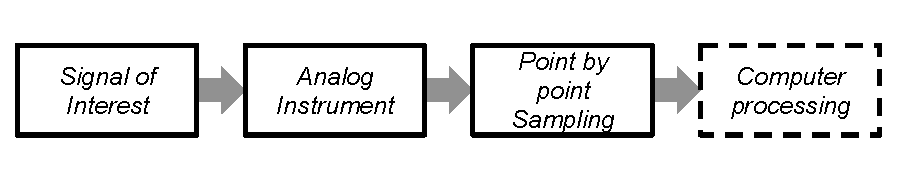
\includegraphics[scale=1]{isomorphicsensorflowchart}
    \caption{A systems view of a traditional sensing scheme. The signal-of-interest is incident upon the analog instrument. The analog instrument forms an isomorphism of the signal which is then periodically sampled point-by-point through an \gls{adc} device. Once the signal is in digital form, post-processing algorithms are often used to perform various tasks such as noise reduction, detection, and classification. Notice that the analog instrument, sampling scheme, and processing are all seperated. }
    \label{fig:isomorphicsesingflowchart}
\end{figure}


\begin{figure}
    \centering
    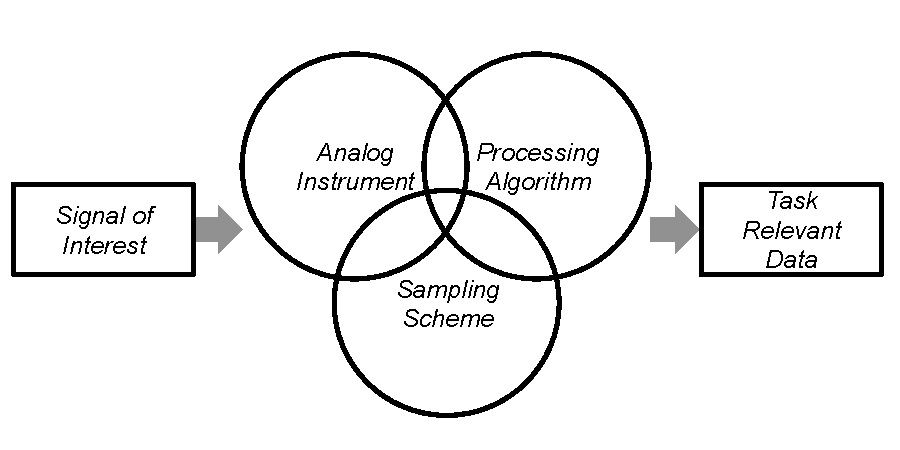
\includegraphics[scale=1]{computationalsensingflowchart}
    \caption{A systems view of a computational sensing scheme. The signal-of-interest is incident upon the analog instrument.  }
    \label{fig:computationalsensingflowchart}
\end{figure}


Rather than a rigorous discussion, this chapter will discuss some of the major developments and concepts in the field of computational sensing on an intuitive level. This will familiarize the reader with important terminology and techniques common in the field of computational sensing. A rigorous discussion with mathematical formalism of the concepts is given in \autoref{chap:Formalism}. This chapter will also discuss some of the challenges I and many other experimentalists and engineers have faced when developing computational sensing prototypes. I will close this chapter with a brief look ahead to the rest of the dissertation. 

%History%%%%%%%%%%%%%%%%%%%%

\section{Isomorphic Sensing}\label{sec:Isomorphic Sensing}

In Greek, the word isomorphic loosely translates to equal in form. Traditional sensors perform isomorphic sensing. In the context of this dissertation, an isomorphic sensor is any sensor which attempts to produce an output signal that resembles the signal-of-interest. In this paradigm, the analog instrument, sampling scheme, and post-processing algorithms are seperated.

We will discuss three important examples of isomorphic sensors: the pinhole camera, the photographic camera and the optical spectrometer (which I will just call a spectrometer from now on, even though there are many instruments called spectromers that not concerned with optical spectra). These sensors have had major roles throughout the history of optics and in the physical sciences so it is natural that they have also been the main focus of computational sensing. Therefore it is important we first understand the isomorphic version of these sensors.

In the photographic camera, the signal-of-interest is the object that is being photographed. This can be anything that is scattering or emitting light, a person, a tree or a distant group of stars. The analog instrument consists of the lens which is designed and fabricated to produce an image that is looks like the object at the \gls{fpa}. The more that the image resembles the object the better the optics. The \gls{fpa} then samples and quantizes the image and produces a digital representation of the object, measurement data. The measurement data is often is post-processed to perform such tasks as noise removal or to locate the object. 


There are two major sub-systems in the photographic camera which determine how well it performs: the optics and the FPA. Ideally, the optics (the analog instrument in this case) will produce a \gls{psf} which is infinitely small in diameter. For example, in a task such as the detection of a star from several neighboring stars in the night sky, if the \gls{psf} is much larger than the center to center seperation of the two stars in the optical image, it will be quite difficult to detect. A careful reader will note that this is the same argument used by Lord Raleigh in proposing his resolution criterion \cite{rayleigh1879investigations}. Even if the \gls{psf} is small enough, the \gls{fpa} must sample at a fine enough pixel-to-pixel spacing, called the \emph{pixel pitch}, to accurately reproduce the intensity variations at the scale which is pertinant to the task. Intuitively, this makes sense because if the image of both stars and the decreased intensity which signifies a certain amount of seperation between the two stars is imaged onto a single pixel, the one cannot ever hope to be able to accurately the detect the star without some other prior or side information. 

The pinhole camera predates the photographic camera over a thousand years, mostly due to it's simplicity. It consists of a small hole and a box which prevents any light except from the pinhole to enter, see Figure \ref{fig:pinholecamera}. The pinhole camera is useful for imaging in parts of the electromagnetic spectrum and particles for which there is no direct analog to refractive lens or reflective mirror. 

\begin{figure}
    \centering
    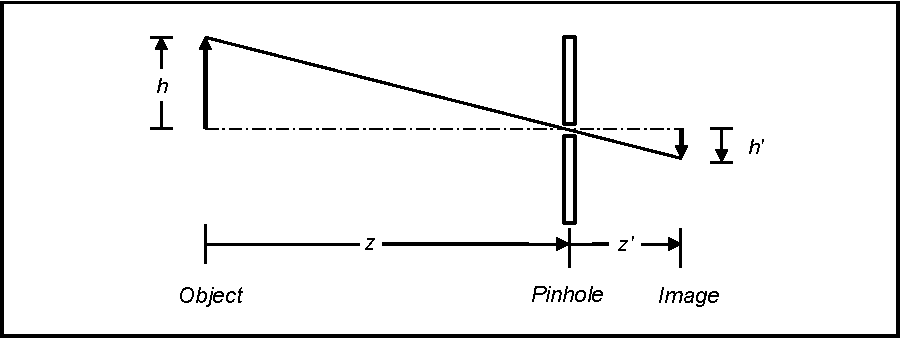
\includegraphics[scale=1]{pinholecamera}
    \caption{A pinhole camera.}
    \label{fig:pinholecamera}
\end{figure}

In the spectrometer, the signal of interest is the spectrum of the object. The optics are designed to take the incoming light and seperate various wavelength components, see Figure \ref{fig:slitspectrometer}. The part of the spectrometer which is used to physically isolate the wavelengths is called a \emph{spectrograph}. The result is a spectral intensity as a function of position at the \gls{fpa}. The \gls{fpa} and post-processing algorithms are used in the same manner as the photographic camera, which is to sample the optical spectrum creating digital version of it and to perform various tasks on the measurement data. For now, we will concentrate on the slit spectrometer, which measurements spectrum at a single point on the object.


\begin{figure}
    \centering
    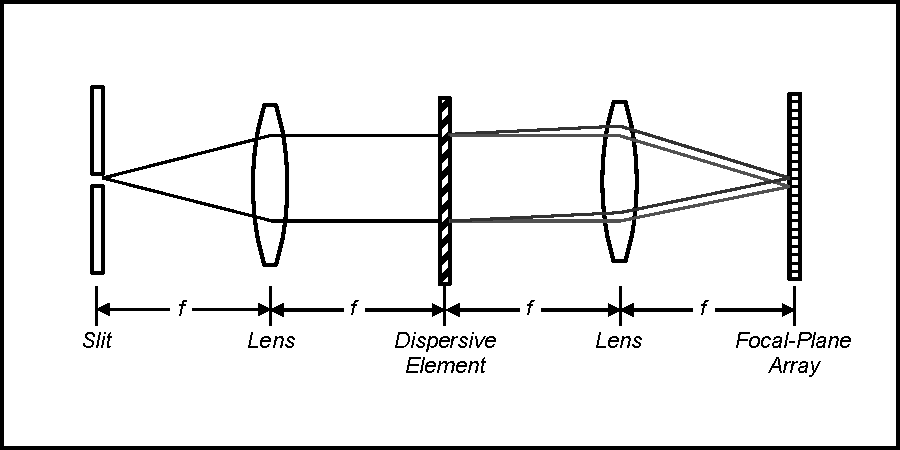
\includegraphics[scale=1]{slitspectrometer}
    \caption{An isomorphic slit spectrometer with a 4F configuration.}
    \label{fig:slitspectrometer}
\end{figure}

In the spectrometer, one of the important performance metrics is \emph{spectral resolution}, which we denote \gls{specres}. The spectral resolution is the smallest difference in wavelength the instrument can discern. Large spectral resolutions can degrade the spectrometers ability to discern important parts of the spectrum. Similarly with the camera, the \gls{fpa} must have a pixel pitch which is small enough in order to correctly sample the variations in the spectrum. 

The point-by-point nature of isomorphic sensing is both a strength and a source of weakness. 

The strength comes from the straightforward and intuitive architecture of the isomorphic sensor. Each subsystem: the optics, the \acrfull{fpa}, and the post-processing can be designed and constructed seperately as long as they meet their individual specifications. As long as the \gls{snr} is sufficient and the sampling rate is high enough we are guaranteed to recover the signal.

One of the weaknessess of the isomorphic approach however is the the ability to measure low \gls{snr} signals. Because the image is sampled in a completely parallel fashion at each exposure, each pixel contributes a certain amount of noise (which is independent of the signal strength). If the noise dominates, the measurement fidelity decreases often forcing the operator to incease the exposure time. For weak signals the exposure time can become prohibitive and for temporally dynamic signals this may lead to a loss of resolution. Indeed, one of the major engineering trade-offs faced by traditional spectrometer designers and users is that when one attempts to increase the light collection (increased slit-width) the spectral resolution \gls{specres} degrades (increases). Similarly, in the pinhole camera, there is a throughput versus spatial resolution trade-off, increasing the size of the pinhole degrades the \gls{psf}.


It would be easy to assume that with the recent revolution in machine learning and statistical signal processing combined with the dramatic increase in computing power that we could simply post-process poor measurments and obtain useful data. However, this isn't possible due to the an important theorem in information theory called the data processing inequality \cite{cover2012elements}. In layman's term it means "garbage in, garbage out".

Another weakness of isomorhic sensing is that the seperation of the analog instrument, the sampling scheme, and the data processing algorithms lead to increased \gls{swap-c}. As we mentioned in the photographic camera, the optics must be designed to produce a small \gls{psf}. For demanding applications, the optical design and fabrication can be the most expensive component of the sensor. While \gls{fpa} prices in the visible have fallen recently, \glspl{fpa} in certain parts of the electromagnetic spectrum can be quite expensive or non-existant \cite{noor2011compressive}.

In many cases, the signal is redundant and high resolution sampling becomes a waste of resources such as data storage and communications bandwidth. A good example is in photography where often the post-processing takes the digital image and applies a compression algorithm which looks for patterns in the signal and reduces the file size, discarding much of the sample data \cite{taubman2012jpeg2000}. 

The isomorphic sensor has served humanity well, however with all the weakness that have been discuss I will now begin to discuss some of major techniques in computational sensing that can be used to address some or all of the issues that I just stated. 

\section{Development of Multiplexing in Sensing}

\emph{Multiplex} sensing allows each measurement sample to be a combination of multiple points of the signal-of-interest. Multiplexing is a powerful tool that can be exploited by the sensor designer to eliminate or relax design trade-offs. 

A simple example which illustrates the usefulness of multiplex sensing is weighing objects. In this example, we are given a 100 sheets of paper. Let's assume that the scale's measurement error is insignificant. Isomorphic measurement sensing means one would need to measure each sheet of paper individually. Requiring 100 measurements. 

Now, let's say the scale's measurement error is on the order of the weight of the sheet. Measuring each sheet invidiually produces a large measurement error. In order to reduce the error to an acceptable \gls{snr} we need to make several measurements per sheet to reduce the error to an acceptable level.

However, we can be a little smarter. We can measure all 100 sheets at the same time. Since the weight of all 100 sheets is much larger than the measurement error of the scale, we can dramatically increase the precision of the measurement. If we can assume that each sheet is the same weight, then we are done. The significant complication occurs when each sheet has a different weight. A single measurement of all 100 sheets is hopeless in this case. We have 1 equation and 100 unknowns. 

What we can do is try measuring different combinations of the 100 sheets, each new combination provides us with a new equation to work with reducing the error. Niavely we might assume that we can randomly choose 100 unique combinations and solve 100 equations from using the algebra we were taught in high school. However, on average random combinations only work well in high \gls{snr} situations. This lead many to begin working on optimal ways to measuring combinations of signals for sensing. 

The weighing problem is directly applicable to the spectroscopy example. As discussed earlier in \autoref{sec:Isomorphic Sensing}, there is trade-off between light collection and spectral resolution. Increasing the slit-width to increase the amount of light has the effect of increasing the spectral resolution \gls{specres}. 

Around the late 1940's and early 1950's, several important inventions demonstrated the effectiveness of multiplexing in spectroscopy. At the time the electronic \gls{fpa} were non-existant. In the slit spectrometer shown in \ref{fig:slitspectrometer}, the \gls{fpa} was actually another slit. To record the intensity at each spectral channel, either the dispersive element or the exit slit had to be mechanically translated, making the measurements even slower by a factor of \gls{numspecchan}, the number of spectral channels of interest. 

Golay was the first to propose multiplexing the slit spectrometer by creating a pattern of binary (1's and 0's) entrance and exit slits \cite{golay1949multi}. The idea borrowed heavily from communications theory which is concerned with the reliable transmission of information over a noisey channel. In the Golay multi-slit spectrometer, the patterns of entrance and exit slits are matched based on mathematically useful properties, this is similar to coding and decoding signals in commucations. The entrance slits act to code the spectrum while the exist slits decodes the coded spectrum. 

Intuitively, the ability to use multiple entrance and exist slits increases the optical throughput of the spectrometer. Fellgett devised an alternative approach to multiplex spectroscopy, the Fourier Transform spectrometer, and was the first to note that multiplex measurements compared to isomorphic measurements improve the signal-to-noise ratio on the order of $ \sqrt{N_{\lambda}}$ \cite{fellgett1958principes}. 

Another example that is pertinant to this dissertation is coded aperture imaging. Coded aperture imaging can be thought of as the multiplexed version of a pinhole camera. As mentioned earlier in \autoref{sec:Isomorphic Sensing}, there is a trade-off between the throughput and spatial resolution. However in many fields, such as high-energy particle imaging, refractive lens and mirrors are non-existant or underdeveloped. By using multiple pinholes the throughput is increased. However, the pattern of the pinholes, which is the code, in this case must be carefully designed to achieve optimal object reconstruction. Fenimore, Canon, and Gottesman were the first to create an elegant solution to coded aperture design called uniformly redundant arrays \cite{fenimore1978coded, gottesman1989new}.

As you can see, multiplexing is a central part of computational sensing. As we will see in \autoref{sec:multiplexingtocompressivesensing} multiplexing is required to solve highly underdetermined sensing problems. We will now discuss the rise of inverse problems in imaging, and how their parallel development to multiplexed optical sensing contributed to the field of computational sensing. While many in the spectroscopy and high-energy particle imaging community were turning to non-isomorphic techniques to eliminate classical design trade-offs, for other fields, isomorphic sensing is non-existant.  

\section{Inverse Problems in Imaging}

What is an inverse problem? And why do they arise in sensing?

It should be noted that often decoding, the task of going from measurement to signal-of-interest, is not necessarily straight forward. And often the coding of the analog signal and decoding are seperately designed in computational sensing. This has become readily apparent because the availible components at the experimentalist disposal limit their ability to implement mathematically optimal codes.

We now turn to what is arguably the most important invention of optical sensing in the last century, the electronic image sensor and how 
it spur the massive growth in computational sensing.

\section{The Digital Imaging Revolution}

Shannon, Nyquist, Wittaker and others established the theory for determining what the pixel spacing must be in order to properly sample the analog signal without loosing any information \cite{shannon1949communication, nyquist1924certain, nyquist1928certain}. 

\section{From Multiplexing to Compressive Sensing}\label{sec:multiplexingtocompressivesensing}

\section{Dissertation Overview}



%\bibliographystyle{IEEEtranS}  
%\bibliography{ThesisBib}

